\subsection{Mission}
Our mission aside from reaching the defined objective is to attract users.
A user will seek us because are unique, because we offer something that
nobody else is offering, because we provide something that they need.
For the user to remain with us, we need to earn their trust We need them to values us, appreciate us, feel a connection with us.
We have to cultivate the relationship, look after our clients and provide satisfaction.

To achieve this satisfaction, we have to have a clear mission - what can we usefully offer that makes us different?
We can consider the characteristics that other products do not have, such as more updated and accurate data,
greater coverage of information or a functionality that does not exist up to now, for example, to use the
information that we offer to solve a daily problem.

Once our mission is defined, we face a series of problems; the user may not be aware that they need a feature that we provide. We have a double challenge, to offer it to users and
to make them realize that it is really necessary, that it helps them in their routine or daily life.

This is where we can make use of the most appropriate marketing techniques to reach our users.
We will have to conduct a study of our target audience, find out what type of advertising they consume and through which channels, so we can approach them in the most appropriate way. Todays market is in a fast paced state of continuous change,
so we must be flexible and adapt to find the perfect formula.

\subsubsection{How to solve it} 
We must study and analyze what the current gaps in the market are, and what needs the user might have that aren't being met.
We need to define the target audience. What do they use in their daily life to keep informed or for entertainment? What type of advertising do they already consume? How can we get closer to them? Keep in mind that we must stay
faithful to the spirit of what we represent, so as well as understanding what advertising fits the user, we should know what kind of advertising
adapts most suitably to our product.
\subsubsection{How we solve it. Aire Guru} 
The mission of Aire Guru is to increase the awareness of the quality of the air.
There are several problems regarding this issue, the first one is user ignorance. Users may not be
aware of the levels of pollution to which they are exposed and may not even know how it pollution can harm them
in the short or long term.

Aire Guru tries to alert them to how air quality influences us, in a way that everyone, independent of their cultural or educational level,
can clearly understand. It aims to make the information, and what that information means, available to everyone. We show how harmful it is to live in a highly polluted area and what the most common sources of pollution
are, so that we can increase awareness and empower users to do something about it.


Aire Guru includes in its glossary the most common medical conditions that may be affected by air pollution, the polluting agents and the sources that produce these agents. It is accompanied by an iconography
which reflects each of the symptoms. \\

\begin{figure}[ht]
    \centering
   \subfigure[Glossary detail]
    {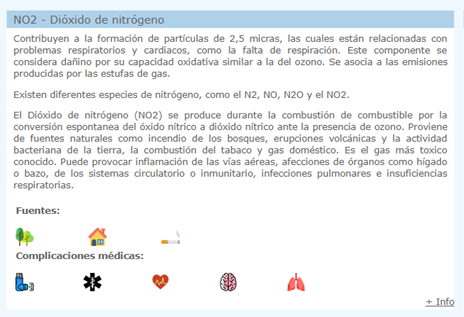
\includegraphics[width=6.2cm  ]{no2_glosary}}
    \hfill
     \subfigure[iconography detail]
     { 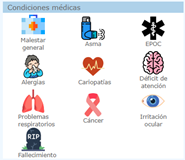
\includegraphics[width=5cm]{iconography}}
  
  \caption{Glossary}
    \end{figure}
\elsparagraph{Evaluation}  
\begin{itemize}
    \done In the survey conducted, users told us that their interest in air pollution had grown. Some of them discovered that they had a medical condition that is affected by the pollution.
    \crossed Air Guru needs more expansion.
    
\end{itemize}
\newpage